\documentclass[../distribution_theory_notes.tex]{subfiles}
\begin{document}
\section{Aula 03 - 23 de Agosto, 2024}
\subsection{Motivações}
\begin{itemize}
 \item Tipos de Conjuntos; 
 \item Convergência em TVS;
 \item Exaustão de abertos.
\end{itemize}
\subsection{Convergência em TVS's}
  Para melhor entendermos a estrutura base da Teoria das Distribuições, ou seja, os Espaços de Fréchet, precisamos dar algumas definições nas duas últimas aulas; com elas, nosso arcabouço teórico atual conta com as noções de: 
 \begin{itemize}
   \item \textbf{\underline{Conjunto Absorvente}:} contém \(\alpha x\) para todo x no conjunto e \(\alpha \) suficientemente pequeno em módulo; 
   \item \textbf{\underline{Conjunto Equilibrado}:} para todo \(|\alpha |\leq 1,\) temos \(\alpha B \subseteq B\);
   \item \textbf{\underline{Conjunto Convexo}:} contém o segmento de reta que liga quaisquer dois pontos dentro de si;
   \item \textbf{\underline{TVS Localmente Convexo}:} a origem possui um SFV conexas;
   \item \textbf{\underline{Família de Seminormas}:} ``normas'' mas que, quando se anulam, não necessariamente foi na origem. Uma família delas é separante quando, juntas, funcionam como uma norma.
 \end{itemize}
   \begin{tcolorbox}[
   skin=enhanced,
   title=Observação,
   fonttitle=\bfseries,
 colframe=black,
   colbacktitle=cyan!75!white, 
   colback=cyan!15,
   colbacklower=black,
 coltitle=black,
   drop fuzzy shadow,
   %drop large lifted shadow
   ]
   Como sabemos, a análise não funciona sem a desigualdade triangular, então, em nossa exploração pelos reinos das distribuições, precisamos de um substituto. Ao termos um conjunto equilibrado e convexo, temos uma substituição da desigualdade triangular; além disso, quando temos um conjunto convexo, equilibrado e absorvente, temos o equivalente à desigualdade triangular para seminormas. 
   \end{tcolorbox}
   Também provamos, em meio a outras coisas nos teoremas da aula passada, que as translações e dilatações são homeomorfismos num TVS arbitrário.
   \begin{figure}[H]
   \begin{center}
   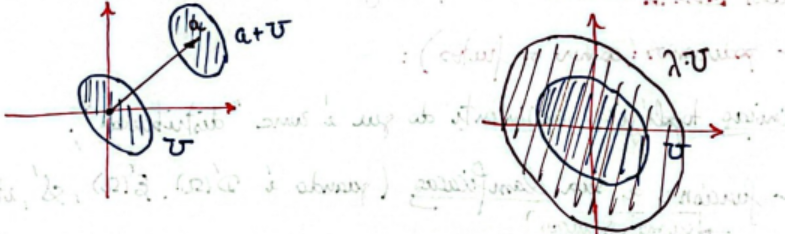
\includegraphics[height=0.8\textheight, width=0.8\textwidth, keepaspectratio]{./Images/trans_dilation_03.png}
   \end{center}
   \caption{em particular, dado um aberto U, a translação \(U+a\) e a dilatação \(\lambda \cdot U\) ambos são abertos, dado que \(\lambda \) é não nulo.}
   \end{figure}

   Terminamos a aula passada com um resultado resumindo tudo, ou quase tudo, que se pode ser dito sobre uma topologia localmente convexa, mas de forma parcial. Hoje, completaremos essa afirmação mostrando a recíproca do que vimos (ainda que de modo temporário, pois substituiremos por \textit{nets}): veremos como ele pode ser usado para ``traduzir'' a convergência de sequências num TVS com topologia gerada por uma família de seminormas, fornecendo, assim, uma ferramenta para construir exemplos de espaços localmente convexos, e finalizaremos a aula exibindo alguns deles. Vale mencionar que o termo ``vizinhança de um ponto x em E'', aqui, será usado para designar um aberto U de E que contém x.

     \begin{tcolorbox}[
     skin=enhanced,
     title=Observação,
     fonttitle=\bfseries,
   colframe=black,
     colbacktitle=cyan!75!white, 
     colback=cyan!15,
     colbacklower=black,
   coltitle=black,
     drop fuzzy shadow,
     %drop large lifted shadow
     ]
     A família de seminormas \(\{p_{\alpha }\}_{\alpha \in L}\) pode ter qualquer cardinalidade -- L pode ser finito, infinito, enumerável, ou não enumerável. Ela é uma família de parâmetros usada para satisfazer as medições dos vetores, ao contrário da norma, que é a única responsável.
     \end{tcolorbox}

    \begin{def*}
      Um conjunto B de um TVS E é dito \textbf{limitado} quando, para toda vizinhança U da origem, \(B\subseteq tU\) para todo t positivo e suficientemente grande; noutras palavras, se existe s positivo tal que 
        \[
          B\subseteq tU,\quad  \forall t\geq s.\quad \square
        \]
    \end{def*}
    O legal dessa definição é que ela \textit{não} depende de métrica alguma, apenas da topologia de E, donde faz sentido dizer que ela é \textbf{\textit{intrínseca}}, superior à definição que envolve o uso das métricas.
    \begin{figure}[H]
    \begin{center}
    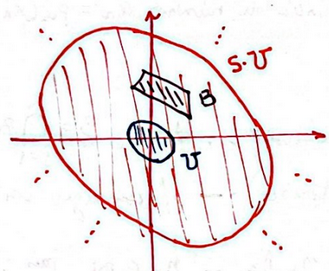
\includegraphics[height=0.5\textheight, width=0.5\textwidth, keepaspectratio]{./Images/bounded_set_03.png}
    \end{center}
    \end{figure}

   \begin{def*}
     Dizemos que uma sequência \(\{x_{n}\}_{n}\) num TVS \((E, \tau )\) \textbf{converge para o vetor x em E}  quando, para toda vizinhança U da origem, existir um natural \(n_{0}\coloneqq n_{0}(U, x)\) tal que, para \(n\geq n_{0}\), temos 
       \[
         x_{n}-x\in U.
       \]
       De forma equivalente, dado uma vizinhança V de x, existe \(n_{0}\) natural tal que, para \(n\geq n_{0}\), temos \(x_{n}\in V\). Em ambos os casos, escrevemos 
         \[
           x_{n}\overbracket[0pt]{\longrightarrow}^{\substack{E \\ n\rightarrow \infty}}X\text{, ou }x_{n}\overbracket[0pt]{\longrightarrow}^{\substack{\tau  \\ n\rightarrow \infty}}\text{, ou } x_{n}\rightarrow x.\square
         \]
   \end{def*}
   A definição equivalente faz sentido pois \(T_{x}:E\rightarrow E\) é homeomorfismo, tal que 
     \[
       U\in \mathcal{B}_{0} \Longleftrightarrow x+U\in \mathcal{B}_{x}.
     \]
    \begin{lemma*}
      Se a topologia de um TVS é dada por uma família \(\{p_{\alpha }\}_{\alpha \in L}\) de seminormas, \(\{x_{n}\}_{n}\) é uma sequência em E e x é um ponto de E, então 
        \[
        x_{n}\overbracket[0pt]{\longrightarrow}^{\substack{E \\ n\rightarrow \infty}}x \Longleftrightarrow p_{\alpha }(x_{n}-x)\overbracket[0pt]{\longrightarrow}^{\substack{\mathbb{R} \\ n\rightarrow \infty}}0,\quad \forall \alpha \in L,
        \]
        ou seja, uma sequência converge para um vetor em E se, e somente se, ela converge passando por todas as seminormas. 

        Além disso, um conjunto B de E é limitado se, e somente se, ele é limitado em todas as seminormas, ou seja, 
          \[
            \sup_{x\in B}p_{\alpha }(x)<\infty,\quad \forall \alpha \in L.
          \]
          Em particular, toda sequência convergente é limitada.
    \end{lemma*}
    \begin{proof*}
       Com efeito, dado \(\varepsilon \) positivo e uma semibola 
         \[
           B = B_{\alpha }(x; \varepsilon ),\; \alpha \in L
         \]
         quaisquer, se supusermos que \(\{x_{n}\}_{n}\) converge para x, então existe um natural \(n_{0}=n_{0}(x, \alpha )\) tal que, quando \(n\geq n_{0}\), 
           \[
             x_{n}\in B \Longleftrightarrow x_{n}\in B_{\alpha }(x; \varepsilon ),
           \]
           ou seja, quando \(n\geq n_{0}\), temos 
             \[
               p_{\alpha }(x_{n}-x)<\varepsilon ,
             \]
             e isto quer dizer que a sequência das seminormas aplicadas a \(x_{n}-x\) converge para zero em \(\mathbb{R}:\)
               \[
                 p_{\alpha }(x_{n}-x)\substack{\mathbb{R} \\ \rightarrow \\ n\to \infty}0.
               \]

               Por outro lado, supondo válida a condição de seminormas, então dada uma vizinhança básica de x como 
                 \[
                   B = \bigcap_{j=1}^{k}B_{\alpha_{j}}(x; \varepsilon ),
                 \]
                 então existem naturais \(n_{1},\dotsc , n_{k}\) tais que, quando \(n\geq n_{j}\), 
                   \[
                     p_{\alpha_{j}}(x_{n}-x)<\varepsilon .
                   \]
                   Logo, colocando \(n_{0}=\max\{n_1, \dotsc , n_{k}\}\), então se \(n\geq n_{0}\), 
                     \[
                       p_{\alpha_{j}}(x_{n}-x)<\varepsilon \Longleftrightarrow x_{n}\in \bigcap_{j=1}^{k}B_{\alpha_{j}}(x; \varepsilon ) = B = x+\bigcap_{j=1}^{k}B_{\alpha_{j}}(0; \varepsilon ).
                     \]
                     Portanto,
                       \[
                         x_{n}-x\in \bigcap_{j=1}^{k}B_{\alpha_{j}}(0;\varepsilon ) \;\&\; x_{n}\rightarrow x 
                       \]
                       em E. A parte sobre conjuntos limitados é deixada como exercício. \qedsymbol
    \end{proof*}
    Para os exemplos, vamos começar simples e ir sofisticando. O exemplo zero e o mais esperado dessa construção é a topologia proveniente de uma norma; neste caso, a família de seminormas é unitária e as semibolas são as bolas usuais segundo essa norma. 

   \begin{example}
     Começando com os exemplos não triviais, sejam X um conjunto qualquer e \(\mathcal{F}(X; \mathbb{C})\) o conjunto de todas as funções complexas definidas em X, lembrando que uma forma de descrever este conjunto é como o produto cartesiano de \(\mathbb{C}\) por \(\mathbb{C}\) cardinalidade de X vezes: 
       \[
         \mathcal{F}(X; \mathbb{C})=\mathcal{C}^{X}=\prod\limits_{x\in X}^{}\mathbb{C}.
       \]

       Aqui, para cada ponto x em X, podemos considerar a seminorma (Verifique!) 
      \begin{align*}
        p_{x}:&\mathcal{F}(X; \mathbb{C})\rightarrow \mathbb{R}\\ 
              &f \mapsto p_{x}(f)\coloneqq |f(x)|.
      \end{align*}
     \begin{figure}[H]
     \begin{center}
     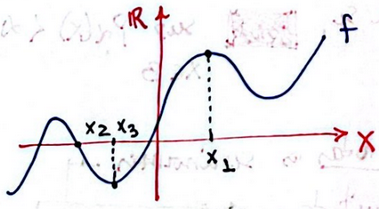
\includegraphics[height=0.5\textheight, width=0.5\textwidth, keepaspectratio]{./Images/complex_seminorms_03.png}
     \end{center}
     \caption{para ilustrar as seminormas, neste caso, \(p_{x_2}(f)=0\) e \(p_{x_{3}}(f)=-p_{x_{1}}(f).\)}
     \end{figure}

      Desta forma, \(\mathcal{F}(X; \mathbb{C})\) torna-se um TVS quando munido da topologia \(\tau \) gerada pela família de seminormas \(\{p_{x}\}_{x\in X}\), a qual é separante! Portanto, \(\tau \) é Hausdorff é, quando X enumerável, \(\tau \) é metrizável; mais explicitamente, se \(X=\mathbb{N}\), então 
        \[
          \mathcal{F}(\mathbb{N}; \mathbb{C}) = \mathbb{C}^{\mathbb{N}},
        \]
        que é exatamente o conjunto das sequências de números complexos.

        Finalmente, pelo lema que provamos, a sequência \(\{f_{n}\}_{n}\) converge para uma função \(f:X\rightarrow \mathbb{C}\) na mesma topologia se, e somente se, 
          \[
            p_{x}(f_{n}-f)\substack{\rightarrow  \\ n\to \infty}, \quad \forall x\in X \Longleftrightarrow |f_{n}(x)-f(x)|\substack{\rightarrow  \\ n\to\infty} 0,\; x\in X,
          \]
          ou seja, quando a sequência \(\{f_{n}\}_{n}\) converge pontualmente para f. Logo, \(\tau \) descreve a topologia d convergência pontual de funções (e toda sequência de Cauchy converge nessa topologia).
   \end{example}
  \begin{example}
    Considere o conjunto das funções contínuas com domínio real e codomínio complexo: 
      \[
        \mathcal{C}(\mathbb{R})\coloneqq \mathcal{C}(\mathbb{R}; \mathbb{C})=\{f:\mathbb{R}\rightarrow \mathbb{C}:\; f\text{ é contínua}\}.
      \]
      Para cada m natural, definimos a seminorma 
     \begin{align*}
       p_{m}:&\mathcal{C}(\mathbb{R})\rightarrow \mathbb{R}\\ 
             &f\mapsto p_{m}(f)\coloneqq \int_{-m}^{m}|f(x)| \mathrm{dx},
     \end{align*}
     que é de fato uma seminorma pelas propriedades das integrais. Além disso, fixada f em \(\mathcal{C}(\mathbb{R})\), temos 
       \[
         p_{1}(f)\leq p_{2}(f)\leq \dotsc \leq p_{m}(f)\leq \dotsc,
       \]
       ou seja, ao aumentar os índices, aumentamos a ``área capturada''. 
      \begin{figure}[H]
      \begin{center}
      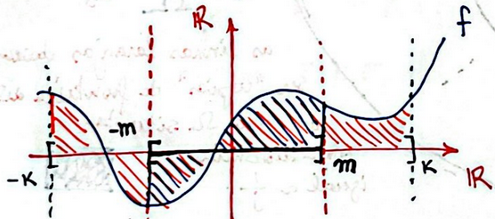
\includegraphics[height=0.5\textheight, width=0.5\textwidth, keepaspectratio]{./Images/integral_seminorms_03.png}
      \end{center}
      \caption{para cada m natural, \(p_{m}(f)\) associa a área sob o gráfico de f no intervalo \([-m, m]\).}
      \end{figure}

      A família de seminormas aqui é \textit{enumerável} e \textit{separante}:
        \[
          \int_{-m}^{m}\underbrace{|f(x)|}_{\mathclap{>0}} \mathrm{dx},\; \forall m\in \mathbb{N} \Rightarrow f(x)=0,\; \forall x\in [-m, m],
        \]
        de modo que a topologia localmente convexa em \(\mathcal{C}(\mathbb{R})\) que essa família define é metrizável... Mas qual a convergência que ela descreve? 

        Quando uma sequência \(\{f_{n}\}_{n}\) converge numa \(p_{m}\), ela converge em todas as normas ``anteriores'', e, quando m é grande suficiente todo \([a, b]\) está contido num \([-m, m]\). Assim, a convergência descrita é a da integral do módulo das funções contínuas, que é exatamente a convergência \(L^{1}\) restrita a \(\mathcal{C}(\mathbb{R})\).
       \begin{figure}[H]
       \begin{center}
         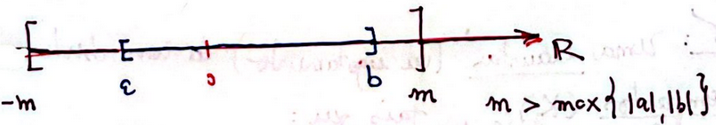
\includegraphics[height=0.5\textheight, width=0.5\textwidth, keepaspectratio]{./Images/natural_interval_03.png}
       \end{center}
       \caption{para encontrar o m suficientemente grande, basta tomar o natural imediatamente seguinte ao máximo \(\max\{|a|, |b|\}\).}
       \end{figure}
  \end{example}

  Antes de darmos continuidade aos exemplos, precisaremos introduzir um conceito novo: o \textit{esgotamento/exaustão} de abertos no espaço euclidiano. Dado um aberto qualquer \(\Omega \) de \(\mathbb{R}^{n}\), para cada j natural, consideramos o conjunto 
    \[
      K_{j}\coloneqq \{x\in \mathbb{R}^{n}:\; |x|\leq j,\; d(x, \mathbb{R}^{n}\setminus{\Omega })>1/j\}.
    \] 
    A imagem que isto forma é a de um monte de compactos que começam dentro de \(\Omega \) e, eventualmente, atingem um ponto que ficam maior que ele; nesse instante, paramos de aumentar, pois exaurimos o aberto inteiro com compactos em seu interior. 
   \begin{figure}[H]
   \begin{center}
   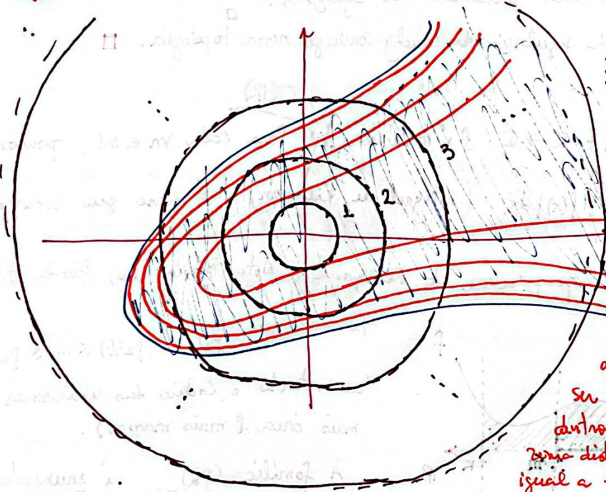
\includegraphics[height=0.8\textheight, width=0.8\textwidth, keepaspectratio]{./Images/big_exhaustion_03.png}
   \end{center}
   \caption{aqui, as linhas laranjas são ``cópias'' da fronteira de \(\Omega \) dentro de \(\Omega \) e situadas a uma distância igual a \(\frac{1}{j}\).}
   \end{figure}
  \begin{figure}[H]
  \begin{center}
  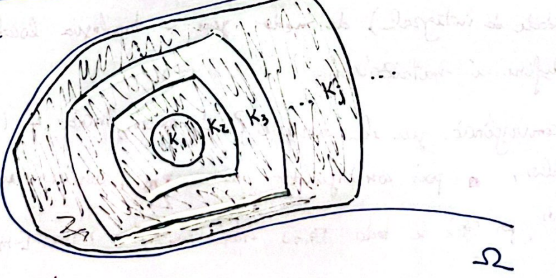
\includegraphics[height=0.8\textheight, width=0.8\textwidth, keepaspectratio]{./Images/small_exhaustion_03.png}
  \end{center}
  \caption{dessa vez, focamos nos conjuntos \(K_{j}\) para ilustração, mostrando como eles vão crescendo até exaustar o conjunto \(\Omega \) da maior forma possível.}
  \end{figure}

 \begin{def*}
   Uma \textbf{exaustão} (ou \textbf{esgotamento}) de um aberto \(\Omega \) de \(\mathbb{R}^{n}\) é uma sequência de \textit{compactos} \(\{K_{j}\}_{j\in \mathbb{N}}\) (a exaustão se refere à sequência) tais que: 
  \begin{align*}
    &(i)\; \Omega =\bigcup_{j=1}^{\infty}K_{j}; \text{ e}\\ 
    &(ii)\; K_{j}\subseteq \mathrm{int}(K_{j+1}),\quad \forall j=1,2,3, \dotsc .\quad \square
  \end{align*}
 \end{def*}
 Como a norma \(|\cdot |:\mathbb{R}^{n}\rightarrow \mathbb{R}\) e  distância a um conjunto \(F\subseteq \mathbb{R}^{n}\), \(d(\cdot , F):\mathbb{R}^{n}\rightarrow \mathbb{R}\), são ambas funções contínuas, os conjuntos 
   \[
     F_{j}=\overline{B}(0; j)\quad\&\quad G_{j}=\{x\in \mathbb{R}^{n}:\; d(x, \mathbb{R}^{n}\setminus{\Omega })\geq 1/j\}
   \]
   são fechados (pela presença do sinal de igual); logo, \(K_{j}\) é fechado. Além disso, cada \(K_{j}\) está contido numa bola fechada \(\overline{B}(0; j)\), tornando-os limitados e, consequentemente, compactos. Note que 
     \[
       F_1\subseteq F_2\subseteq \dotsc \subseteq F_{j}\subseteq \dotsc \quad\&\quad G_1\subseteq G_2\subseteq \dotsc \subseteq G_{j}\subseteq
     \]

     Assim, dado um ponto x em \(\Omega \) e escolhendo \(j_1, j_2\) naturais tais que 
       \[
         |x|\leq j_1 \quad\&\quad d(x, \mathbb{R}^{n}\setminus{\Omega })\geq \frac{1}{j_2},
       \]
       tomando \(j_{x}\coloneqq \max\{j_1, j_2\}\), vê-se que \(x\in K_{j_{x}}\).
        \begin{tcolorbox}[
        skin=enhanced,
        title=Observação,
        fonttitle=\bfseries,
      colframe=black,
        colbacktitle=cyan!75!white, 
        colback=cyan!15,
        colbacklower=black,
      coltitle=black,
        drop fuzzy shadow,
        %drop large lifted shadow
        ]
        A existência do \(j_2\) acima é garantida porque \(\mathbb{R}^{n}\setminus{\Omega }\) é fechado e x não pertence a \(\mathbb{R}^{n}\setminus{\Omega }\), pois \(\Omega \) é aberto e, quando F é fechado, \(d(x, F)= 0\) equivale a x pertencer a F por definição.
        \end{tcolorbox}

        Finalmente, se 
        \[
          |x|\leq j<j+1 \quad\&\quad d(x, \mathbb{R}^{n}\setminus{\Omega })\geq \frac{1}{j} >\frac{1}{j+1},
      \]
      então x pertence ao conjunto \(\Omega _{j+1}\) definido por 
        \[
          \Omega_{j+1}\coloneqq \biggl\{x\in \mathbb{R}^{n}:\; |x|<j+1,\; d(x, \mathbb{R}^{n}\setminus{\Omega })>\frac{1}{j+1}\biggr\},
        \]
        e fica de exercício verificar que \(\Omega_{j+1}=\mathrm{int}(K_{j+1})\). Portanto, além de termos dado sentido à definição acima, provamos a 
       \begin{prop*}
         Todo aberto \(\Omega \) de \(\mathbb{R}^{n}\) possui uma exaustão.
       \end{prop*}


\end{document}
